\documentclass[11pt,a4paper]{ctexart}
\usepackage[margin=1.72cm]{geometry}
\usepackage{amsmath,amssymb,bm}
\usepackage{booktabs,graphicx,xcolor,xurl,hyperref,array,float,tabularx}
\hypersetup{colorlinks=true,linkcolor=blue,urlcolor=blue,citecolor=blue}
\setlength{\parindent}{2em}
\setlength{\parskip}{0.20em}
\newcommand{\norm}[1]{\left\lVert #1\right\rVert}
\newcommand{\med}{\operatorname{median}}
\newcolumntype{P}[1]{>{\raggedright\arraybackslash}p{#1}}
\newcolumntype{Y}{>{\raggedright\arraybackslash}X}
\title{Task06：Pfeiffer IMU--UWB代码复现与无真值公平对比}
\author{作者原协议、去运行时真值协议与XY/三维双口径审计}
\date{2026年8月3日}

\begin{document}
\pagestyle{plain}
\maketitle

\begin{abstract}
TU Delft数据集对应的2021 RA-L工作公开了MIT源码；同作者的2023 IMAV和
2025 IJMAV工作提出动态步长及开关变量异常拒绝，但未找到其LS/Newton/SVOR
实现。本轮固定2021作者源码提交\texttt{955360a...}，重放12条TWR日志、
3种协议、10个随机种子，共360个任务。作者原协议复现MHE/EKF三维RMSE均值
$0.201/0.235$ m。切断OptiTrack派生高度及真值残差权重，并与Task06统一为
逐锚LOSO标定、首帧位置初始化、全轨迹计分后，作者MHE/EKF变为
$0.339/0.321$ m，Task06 InEKF为$0.334$ m。Task06的XY均值$0.170$ m优于
作者MHE的$0.190$ m，但差于作者EKF的$0.161$ m。因此当前结果达到作者MHE
的公平三维量级，却不能宣称超过全部同数据集研究。
\end{abstract}

\section{论文链与代码边界}

\begin{table}[H]
\centering\small
\caption{三篇同作者论文的关系与可复现性。}
\begin{tabularx}{\textwidth}{P{1.7cm}P{3.7cm}YP{3.2cm}}
\toprule
年份 & 方法主线 & 重点问题 & 公开实现\\
\midrule
2021 & 单步固定步长SG+RANSAC & 重尾UWB、少锚点、微型飞行器机载计算 & 有；本轮精确复现\\
2023 & line search/Newton+SVOR & 固定步长随量测数变化失稳；RANSAC成本高 & 未找到\\
2025 & 2023期刊化扩展；Newton+SVOR机载验证 & 加入ToF高度/光流及协方差权重，完整验证 & 未找到\\
\bottomrule
\end{tabularx}
\end{table}

2021将完整MHE简化为忽略过程噪声的output-error问题，只估计位置与机体速度：
\begin{equation}
J(\xi_{t-N})=\mu\norm{\xi_{t-N}-\bar\xi_{t-N}}^2
+\sum_{k=t-N}^{t}\sum_i
\norm{y_{i,k}-\mathcal H_{i,k}(\xi_{t-N})}^2,
\label{eq:paper-cost}
\end{equation}
并每次只执行
\begin{equation}
\hat\xi_{t-N}=\bar\xi_{t-N}-\alpha\nabla J(\bar\xi_{t-N}).
\label{eq:fixed-step}
\end{equation}
姿态由互补滤波器提供。2023指出梯度是所有量测项之和，量测数变化导致
$\norm{\nabla J}$变化；4锚合适的固定$\alpha$可能在8锚时失稳。line search
从$\{0.5,0.8,1,1.25,2\}\alpha$选择最低代价候选，Newton法则用
$(\mathrm D^2J)^{-1}\nabla J$给出分方向步长。

SVOR为每个量测引入
\begin{equation}
\operatorname{sig}(s_{i,k})=\frac{1}{1+e^{-s_{i,k}}},
\end{equation}
在残差项中乘该权重，同时惩罚$s_{i,k}$偏离启用先验。其目标是以连续优化替代
RANSAC反复抽样。论文8锚TWR图中各MHE精度几乎不可区分；改善主要是不同量测数
下的成功率与计算成本，而非显著降低8锚RMSE。

\section{作者原协议中的真值路径}

2021批处理显式开启高度观测，日志回放构造
\begin{equation}
z_k^{\rm pseudo}=z_k^{\rm OptiTrack}(1+\varepsilon_k),
\qquad\varepsilon_k\sim\mathcal N(0,0.02^2),
\label{eq:oracle-alt}
\end{equation}
并送给MHE与EKF。它不是日志中的独立气压计或ToF。回放还计算
\begin{equation}
e_{k,i}^{\rm twr}=\widetilde\rho_{k,i}
-\norm{a_i-p_k^{\rm OptiTrack}},
\label{eq:oracle-range}
\end{equation}
以最近窗口标准差设置量测\texttt{stdDev}。该标准差被作者EKF使用；检查
2021 MHE源码可见式\eqref{eq:paper-cost}及RANSAC均未读取\texttt{stdDev}，
故MHE的主要oracle帮助是式\eqref{eq:oracle-alt}，不能把两条路径对MHE的影响
等量描述。

这不表示作者伪造结果：论文模型允许独立barometer/ToF高度，2025真实机载实验
也使用Flow Deck ToF。公平性问题仅在于不能把由评分真值生成的离线高度协议，与
纯IMU+TWR的三维数值不加说明地排名。

\section{本轮无运行时真值协议}

作者目录保持不改；适配器关闭高度量测，并把真值残差函数替换为冻结尺度。对第
$j$条待测日志，只用其余11条训练日志估计
\begin{align}
\hat b_i&=\med_{k\in\mathcal D_{-j}}e_{k,i},\\
\hat\sigma_i&=\operatorname{clip}\!\left(
1.4826\med_{k\in\mathcal D_{-j}}|e_{k,i}-\hat b_i|,
0.08,0.35\right)\ {\rm m},
\label{eq:loso}
\end{align}
测试时使用$\rho_{k,i}=\widetilde\rho_{k,i}-\hat b_i$和冻结$\hat\sigma_i$。
双方均以首帧OptiTrack位置初始化并对$t\ge0$完整轨迹计分。

首帧位置仍是真值初始化，LOSO仍是监督式传感器标定；但待测日志运行过程中不再
注入位置、高度或在线噪声真值。该协议可公平比较现有两套代码，但不能包装成完全
无外部标定的跨场景盲测。

\section{复现结果}

\subsection{作者代码协议消融}

\begin{table}[H]
\centering\small
\caption{作者代码12日志$\times$10种子结果，单位：m。}
\begin{tabular*}{\textwidth}{@{\extracolsep{\fill}}llrrrrr@{}}
\toprule
协议 & 方法 & 3D均值 & 3D中位 & XY均值 & z均值 & 成功\\
\midrule
作者原协议 & MHE & 0.201051 & 0.201250 & 0.191061 & 0.061595 & 120/120\\
作者原协议 & EKF & 0.235375 & 0.234154 & 0.232630 & 0.035726 & 120/120\\
无真值/无偏差标定 & MHE & 0.563604 & 0.578655 & 0.187121 & 0.530934 & 20/120\\
无真值/无偏差标定 & EKF & 0.558660 & 0.577495 & 0.182602 & 0.527470 & 20/120\\
无真值/LOSO & MHE & 0.338650 & 0.318420 & 0.189810 & 0.275932 & 110/120\\
无真值/LOSO & EKF & \textbf{0.321290} & \textbf{0.313002} & \textbf{0.161072} & 0.274212 & \textbf{120/120}\\
\bottomrule
\end{tabular*}
\end{table}

\begin{figure}[H]
\centering
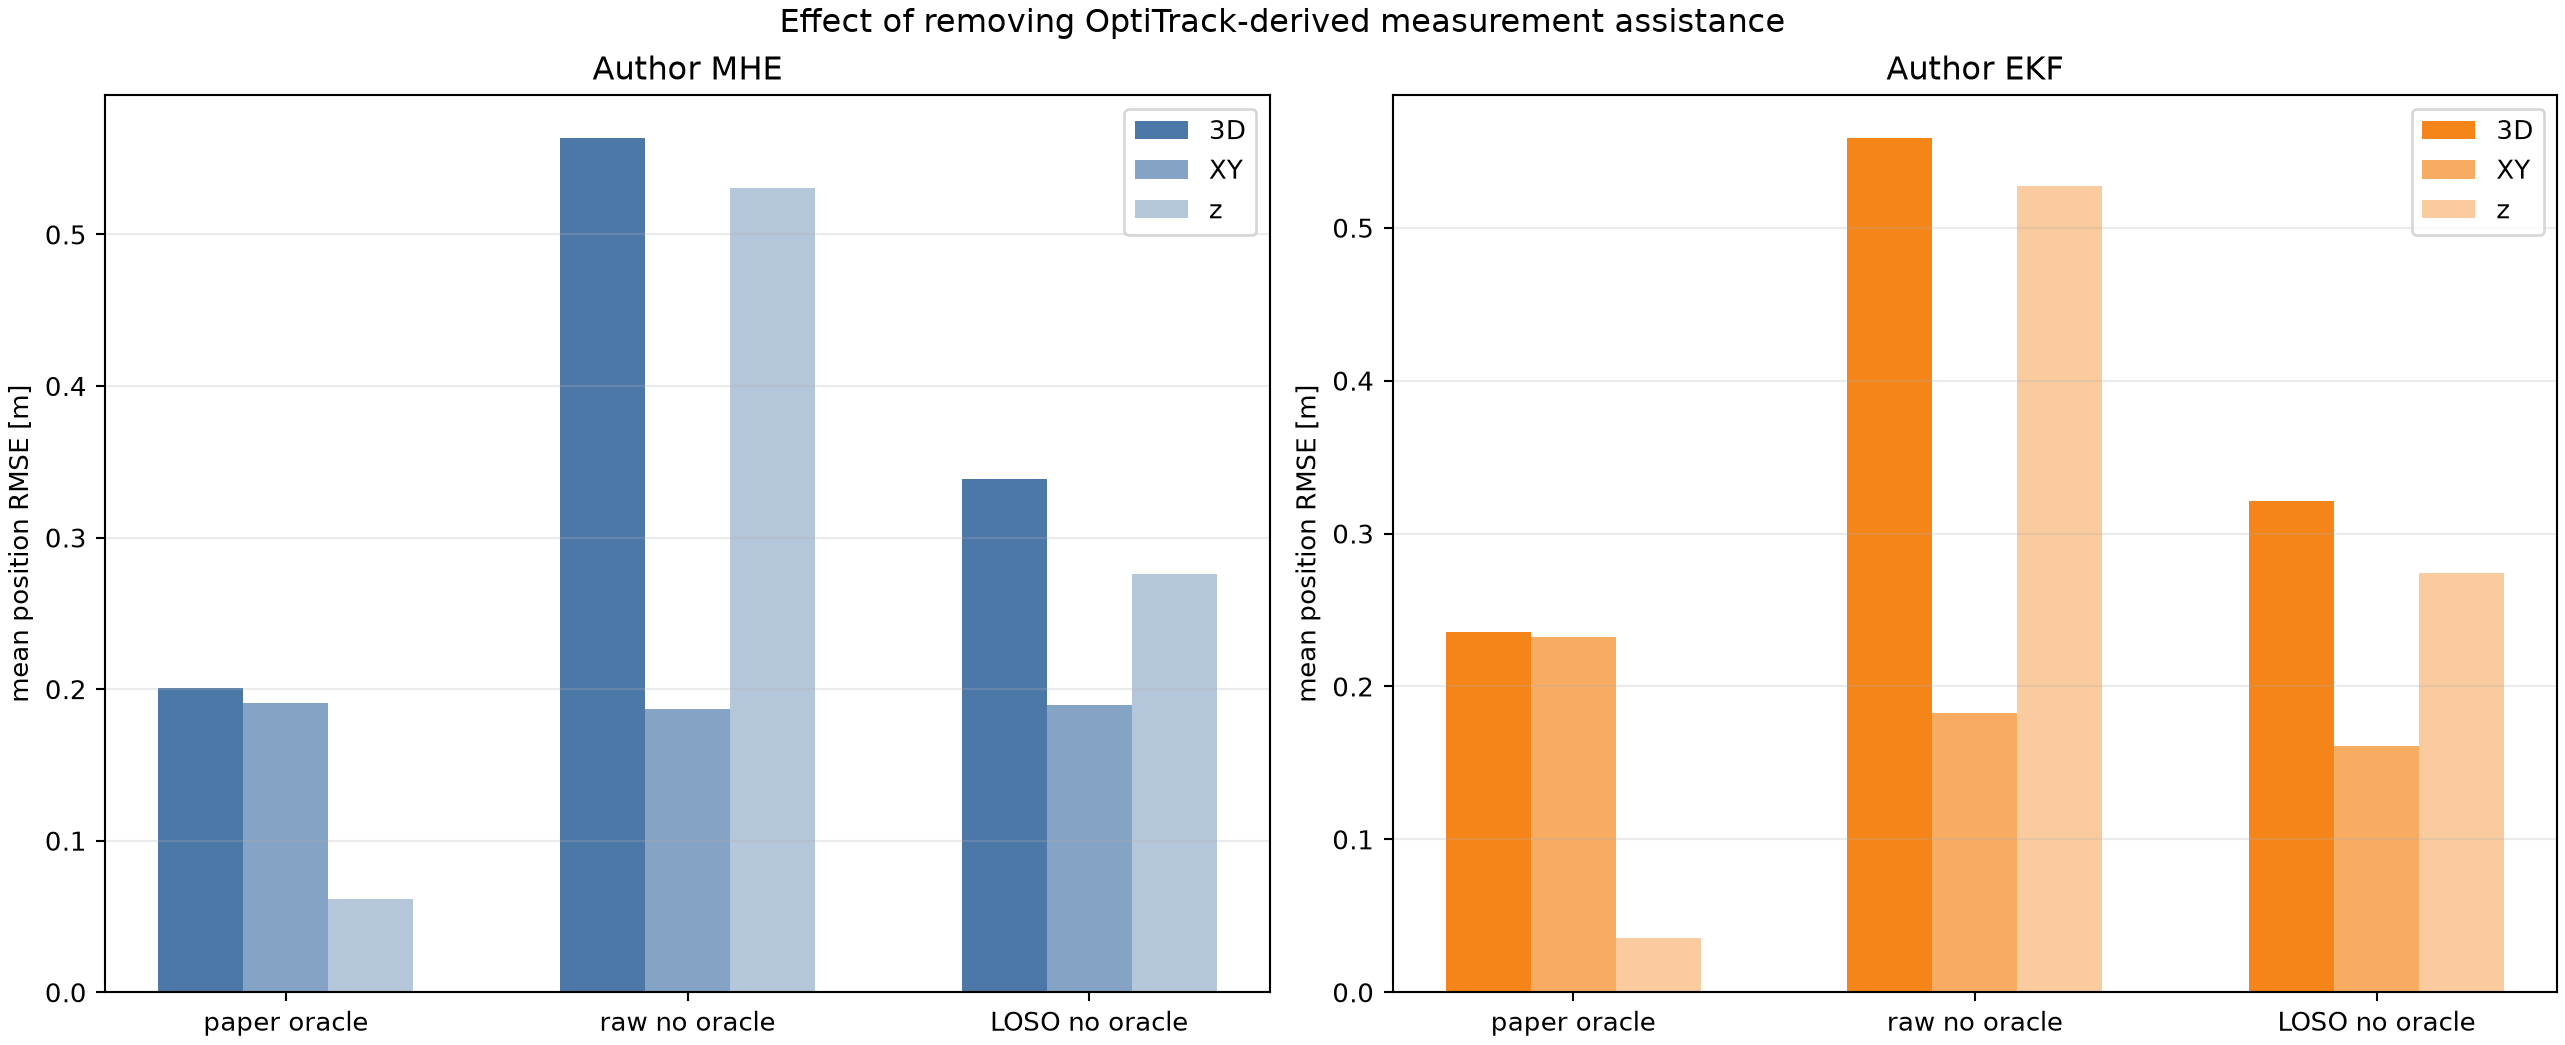
\includegraphics[width=\textwidth]{../imu-uwb-inekf-state-augment/results/task06_author_fair_compare/truth_assistance_ablation.png}
\caption{移除OptiTrack派生量测后的3D、XY与z变化。XY基本不变，退化集中在z。}
\label{fig:oracle-ablation}
\end{figure}

原协议数值与论文图读数$0.20/0.23$ m一致。去真值且不做偏差标定时，MHE/EKF
的XY仅小幅变化，z却增到约$0.53$ m；逐锚LOSO把z降到约$0.275$ m，但垂直
误差仍主导。MHE的10次失败均来自同一star序列，失败没有从精度统计删除。

\subsection{与Task06的公平三维及XY结果}

对每条轨迹定义
\begin{align}
\operatorname{RMSE}_{XY}
&=\sqrt{\frac1N\sum_k[(\hat x_k-x_k)^2+(\hat y_k-y_k)^2]},\\
\operatorname{RMSE}_{3D}^2
&=\operatorname{RMSE}_{XY}^2+\operatorname{RMSE}_{z}^2.
\end{align}

\begin{table}[H]
\centering\small
\caption{相同无运行时真值LOSO协议的12日志聚合，单位：m。}
\begin{tabular*}{\textwidth}{@{\extracolsep{\fill}}lrrrrr@{}}
\toprule
方法 & 3D均值 & 3D中位 & XY均值 & XY中位 & z均值\\
\midrule
作者MHE & 0.338650 & \textbf{0.318420} & 0.189810 & 0.189320 & 0.275932\\
作者EKF & \textbf{0.321290} & \textbf{0.313002} & \textbf{0.161072} & \textbf{0.165110} & \textbf{0.274212}\\
Task06 direct & 0.334476 & 0.332875 & 0.171259 & 0.174492 & 0.283950\\
Task06 InEKF & 0.333703 & 0.328305 & 0.170033 & 0.172807 & 0.283201\\
Task06 lifted & 0.361756 & 0.357657 & 0.170750 & 0.173223 & 0.317015\\
\bottomrule
\end{tabular*}
\end{table}

Task06 InEKF相对作者MHE：3D逐序列赢$8/12$，均值低$4.95$ mm，但中位数
高$9.89$ mm；XY赢$12/12$，均值低$19.78$ mm。相对作者EKF：3D和XY都
只赢$1/12$，均值分别高$12.41/8.96$ mm。

\begin{figure}[H]
\centering
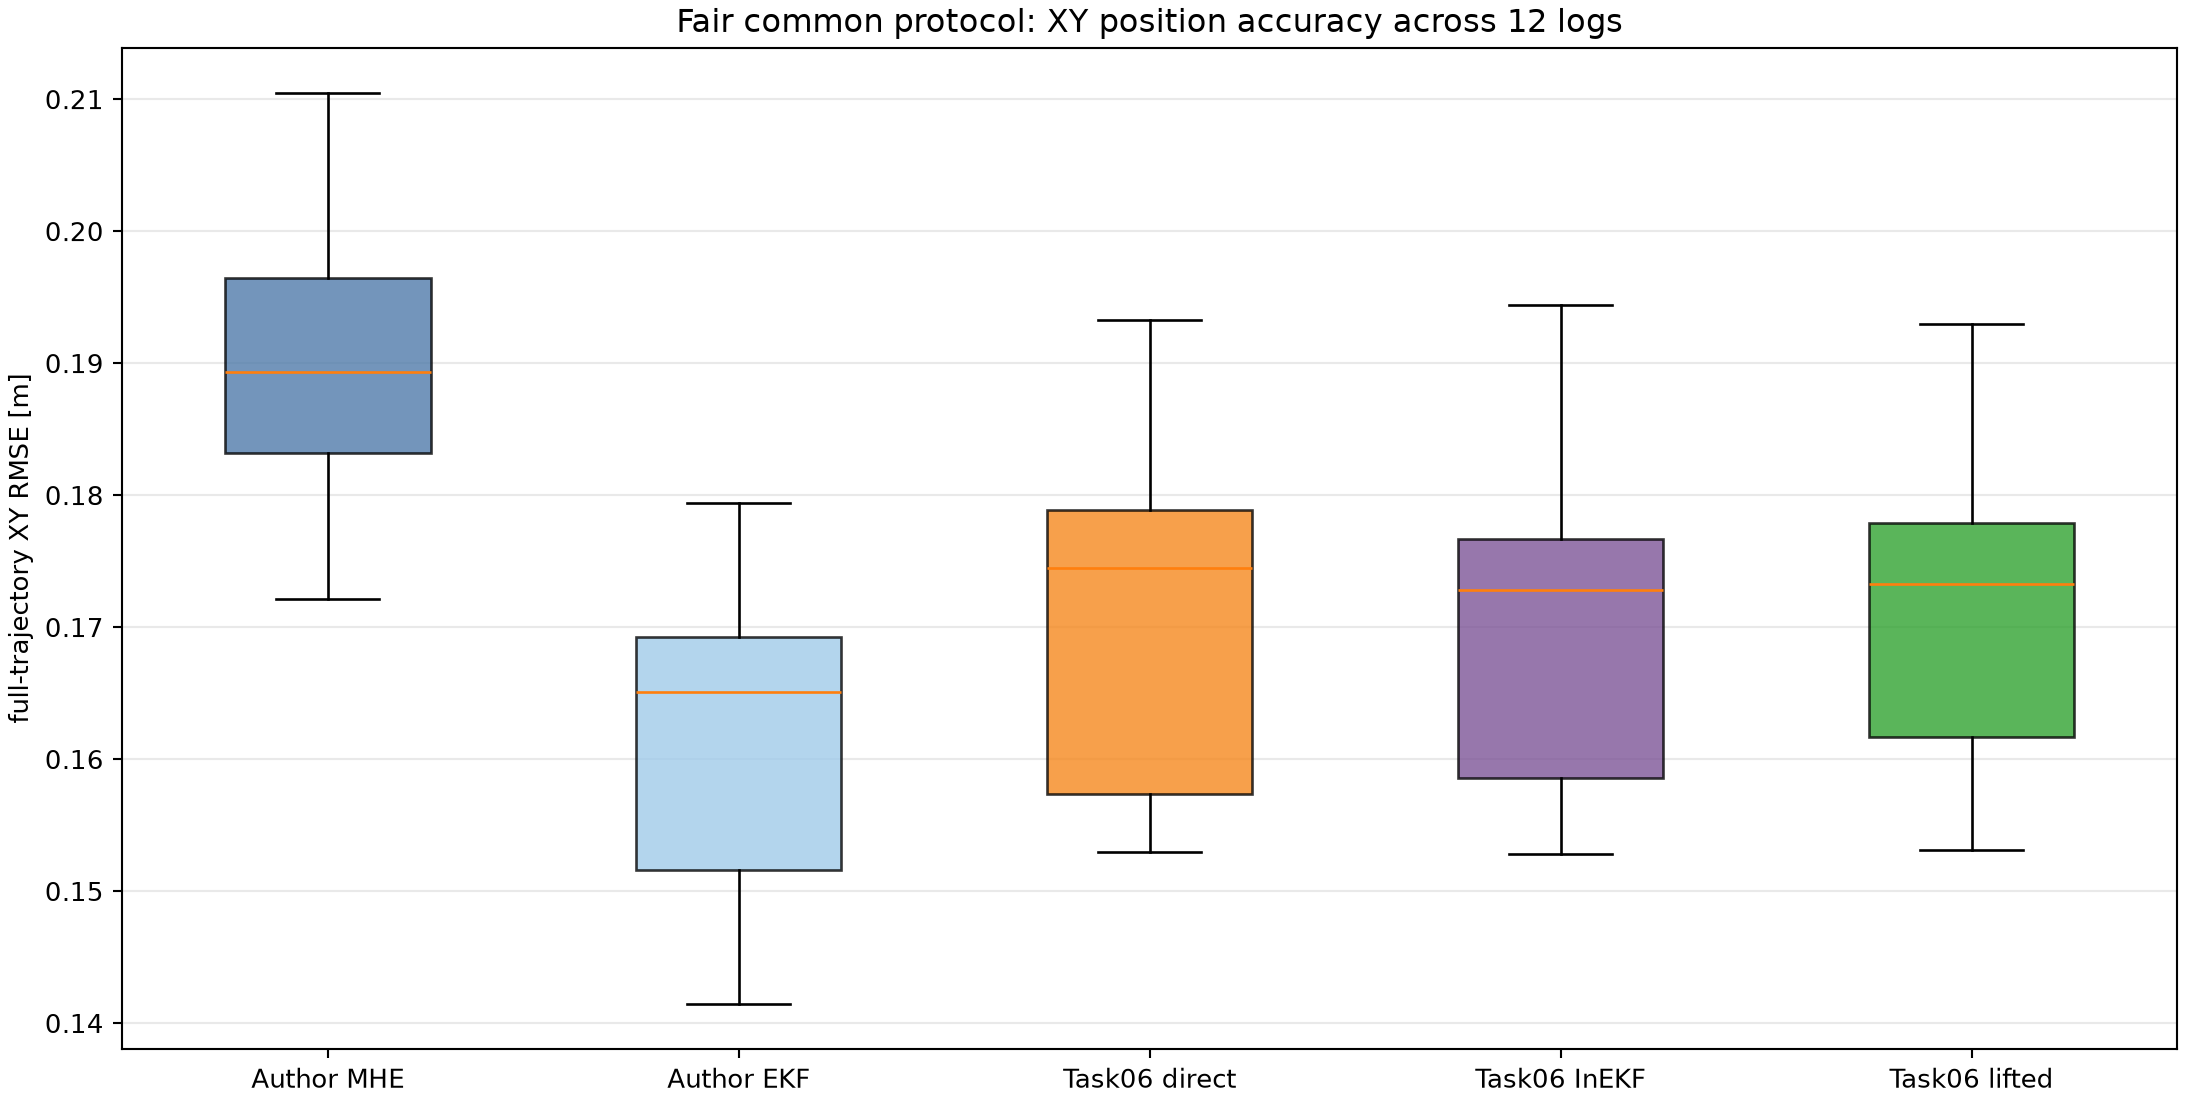
\includegraphics[width=0.92\textwidth]{../imu-uwb-inekf-state-augment/results/task06_author_fair_compare/fair_xy_comparison.png}
\caption{无运行时真值、共同LOSO协议下的12日志XY RMSE。}
\label{fig:fair-xy}
\end{figure}

\begin{figure}[H]
\centering
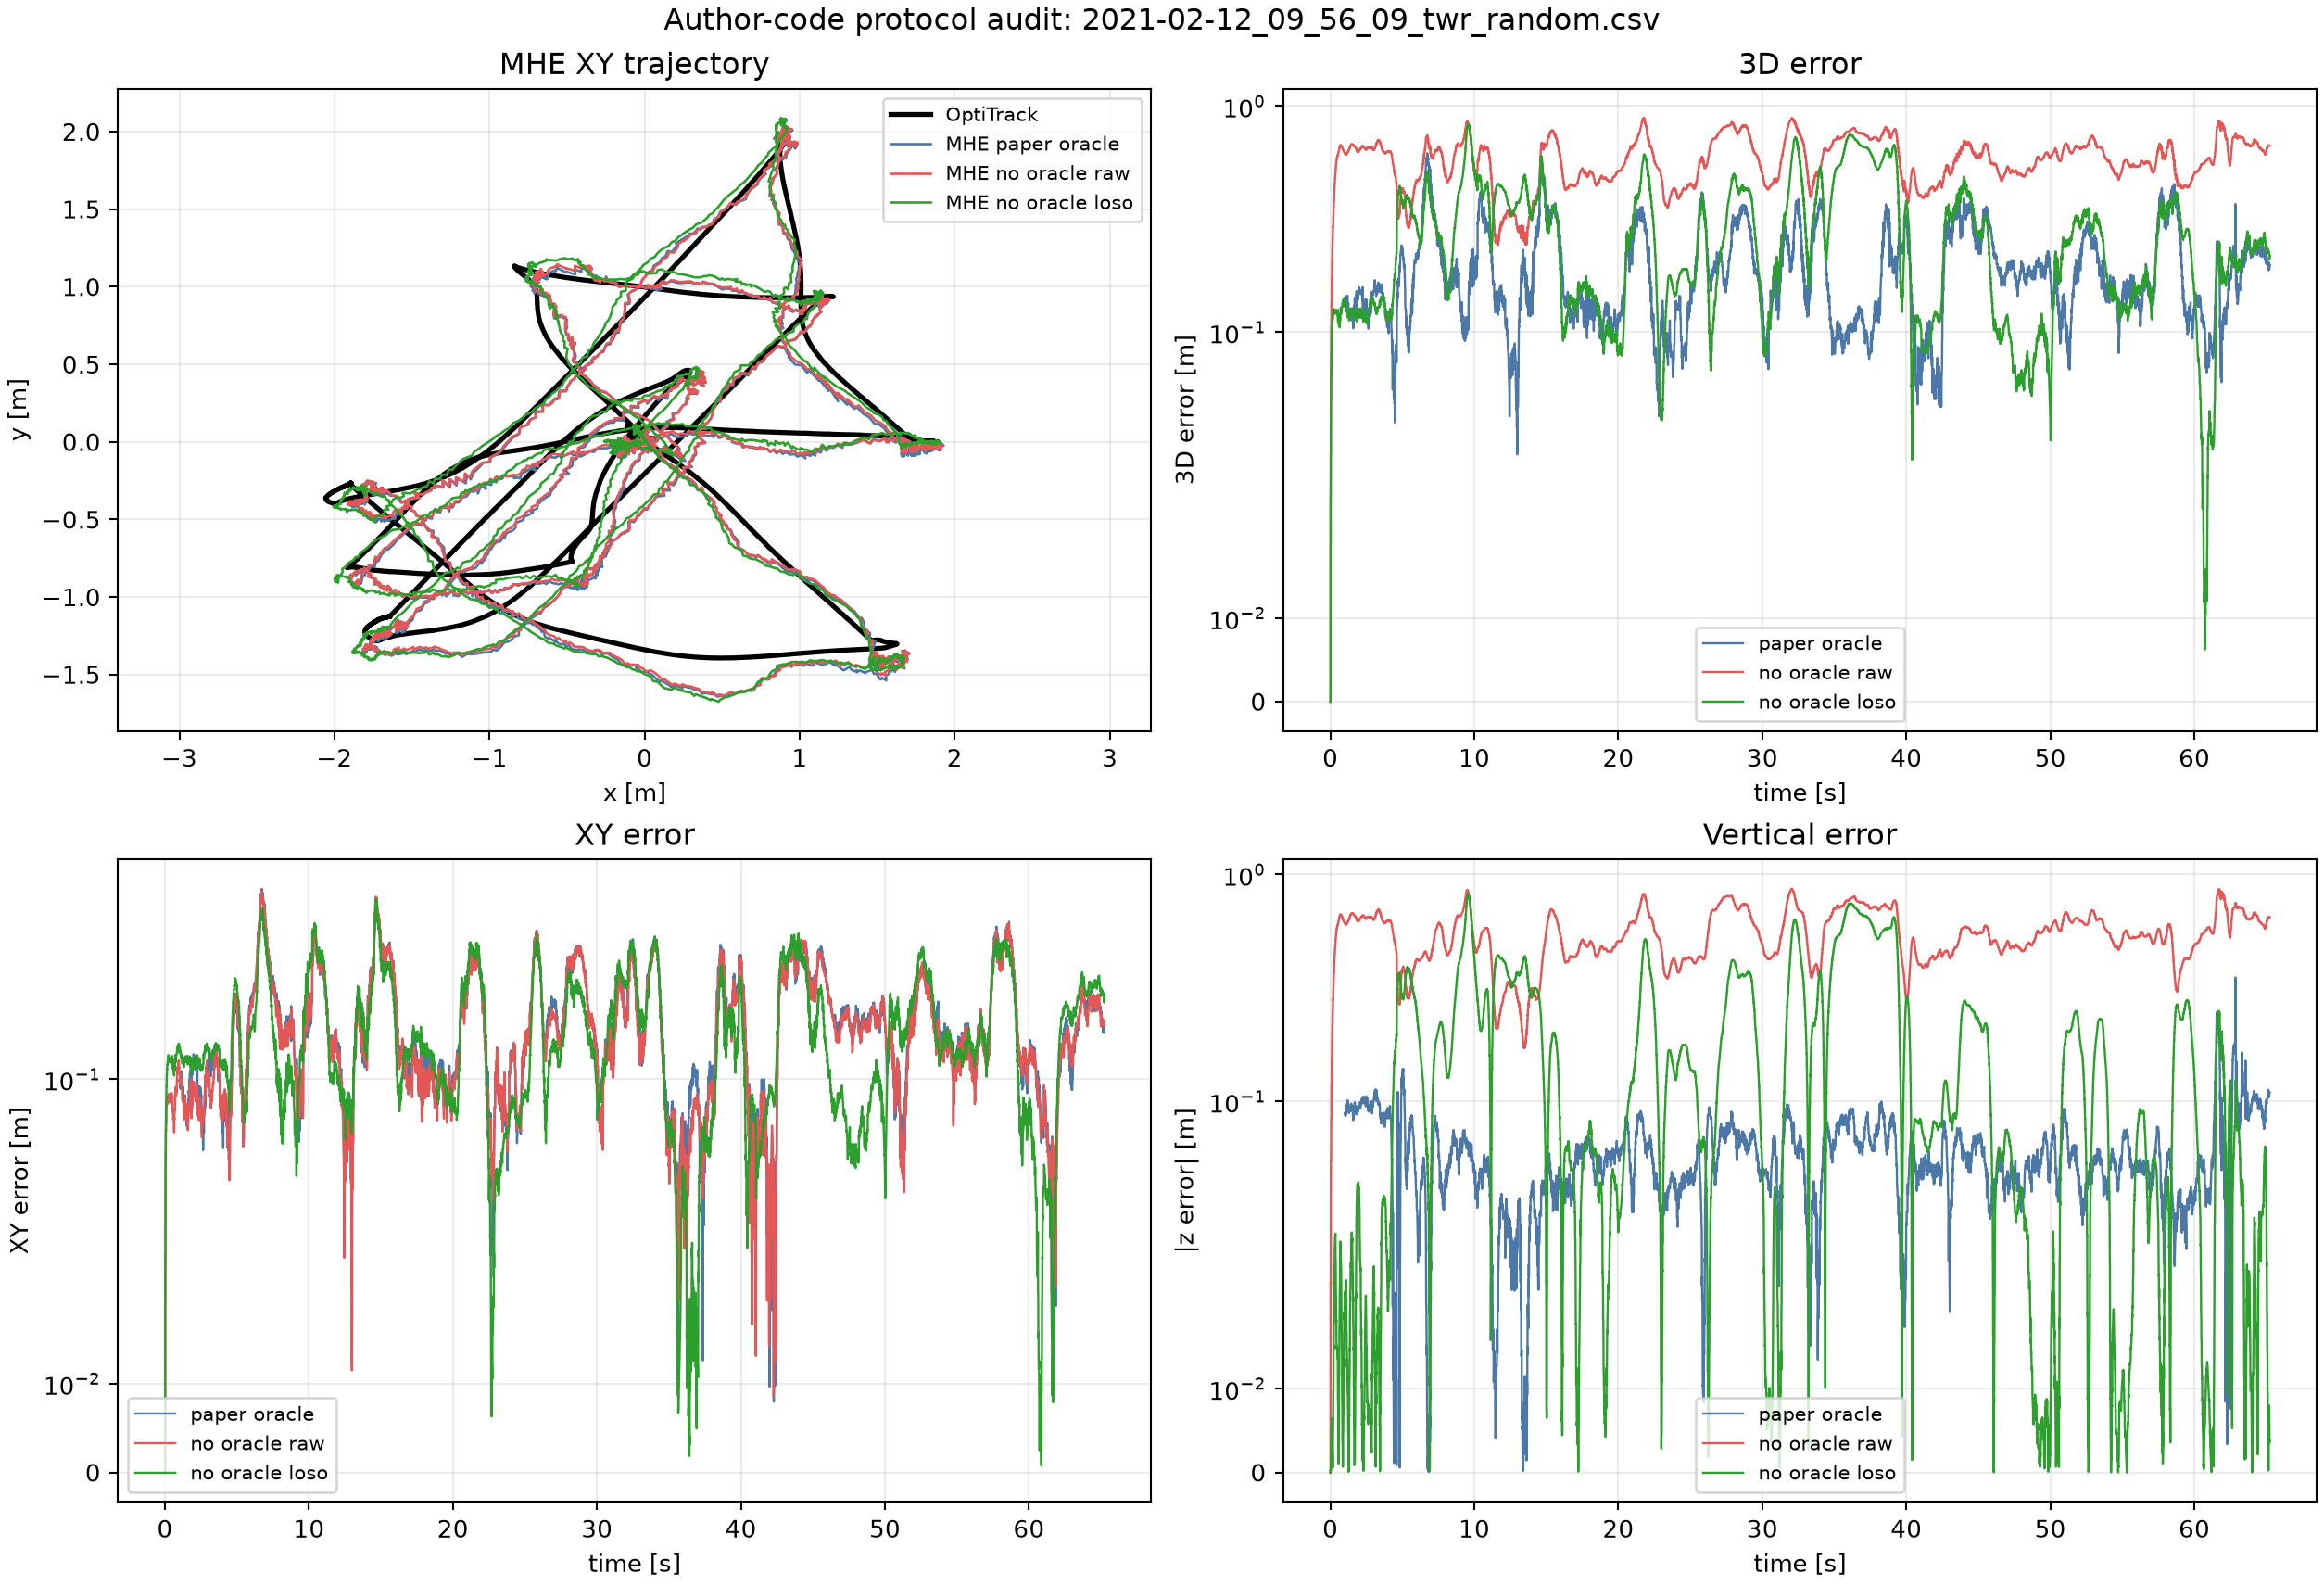
\includegraphics[width=\textwidth]{../imu-uwb-inekf-state-augment/results/task06_author_fair_compare/representative_protocols.png}
\caption{代表轨迹协议审计。三组MHE的XY轨迹接近，主要差异为垂直误差。}
\label{fig:trace}
\end{figure}

\section{可成立的比较结论与检索边界}

当前Task06已达到作者2021 MHE的公平三维量级，并在XY明显优于该MHE；但是作者
仓库中的EKF在相同协议下三维和XY都更好。因此不能宣称本项目已超过所有同数据集
研究。2023/2025没有可审计源码，且完整调参与离线真值路径不明；将论文公式自行
重写可以做方法探索，却不足以给出可靠的作者算法排名。

截至2026-08-03，TU Delft数据门户只列2021原论文为关联输出，DataCite只记录
数据集补充2021论文。对精确DOI、文件名、字段及2021论文16个OpenAlex引用作品
逐项检查后，未核实到独立第三方在这12条TWR日志上报告可直接复核的IMU+UWB
轨迹RMSE。2023与2025是同一作者链的后续，不是独立团队复现；该结论受检索索引
覆盖范围限制，不能证明所有未索引学位论文或私有代码都不存在。

实现产生720行有限方法结果，无真值协议中运行时真值标志均为假。单元测试覆盖
协议开关、三维/XY/z恒等式和LOSO索引。作者上游工作树为空；全部图以原分辨率检查，
未见NaN、轨迹断裂、错位或裁切。

\section*{来源}

\begin{itemize}
\item 数据与代码说明：\url{https://research.tudelft.nl/en/datasets/data-underlying-the-publication-a-computationally-efficient-movin/}
\item 2021论文：\url{https://doi.org/10.1109/LRA.2021.3095519}
\item 作者代码：\url{https://github.com/SUPfeiffer/uwb-simulator}
\item 2023论文：\url{https://www.imavs.org/papers/2023/10.pdf}
\item 2025论文：\url{https://doi.org/10.1177/17568293251340100}
\end{itemize}

\end{document}
